% Author: Izaak Neutelings (November 2020)
\documentclass[border=3pt,tikz]{standalone}
\usepackage{physics}
\usepackage{tikz}
\usepackage[outline]{contour} % glow around text
\tikzset{>=latex}
\contourlength{0.9pt}

\colorlet{mydarkblue}{blue!40!black}
\colorlet{myblue}{blue!30}
\colorlet{myred}{red!65!black}
\colorlet{vcol}{green!45!black}
\colorlet{watercol}{blue!80!cyan!10!white}
\colorlet{darkwatercol}{blue!80!cyan!80!black!30!white}
\tikzstyle{water}=[mydarkblue,top color=watercol!90!black!80,bottom color=watercol!90!black!90,middle color=watercol!80,shading angle=10]
\tikzstyle{air}=[mydarkblue,top color=watercol!90!black!6,bottom color=watercol!90!black!6,middle color=watercol!6,shading angle=0]
\tikzstyle{vvec}=[->,very thick,vcol,line cap=round]
\tikzstyle{force}=[->,myred,very thick,line cap=round]
\tikzstyle{width}=[{Latex[length=3,width=3]}-{Latex[length=3,width=3]}]

\begin{document}

% VENTURI EFFECT
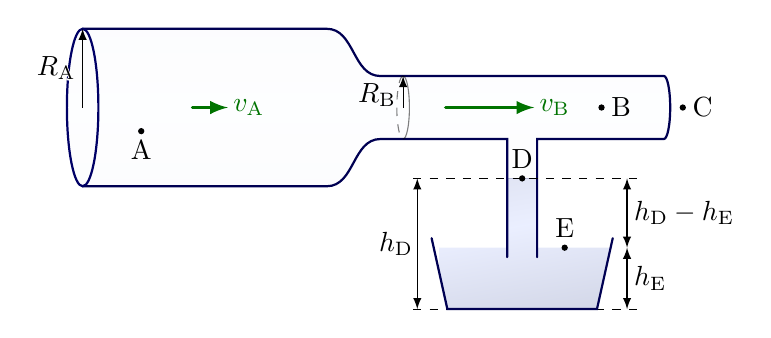
\begin{tikzpicture}
  \def\L{3.1}         % large pipe length
  \def\l{3.6}         % small pipe length
  \def\m{0.22*\L}     % length pipe middle
  \def\Rx{0.20}       % big pipe vertical radius right
  \def\Ry{1.00}       % big pipe vertical radius right
  \def\rx{0.08}       % small pipe horizontal radius left
  \def\ry{0.40}       % small pipe vertical radius left
  \def\t{0.19}        % vertical pipe radius
  \def\h{1.5}         % vertical pipe height
  \def\d{0.12}        % vertical pipe depth in water
  \def\y{1.0}         % height fluid column
  \def\W{2.3}         % width bath top
  \def\w{1.9}         % width bath bottom
  \def\H{0.9}         % height bath
  \def\v{0.45}        % velocity magnitude
  \def\xr{\L+\m+0.08*\l} % ring x position
    
  % WATER
  \draw[dashed] (\L+\m+0.115*\l,-\ry-\h+2*\d-\H) --++ (0.79*\l,0);
  \begin{scope}
    \clip (\L+\m+\l/2-\W/2,-\ry) --++ (0,-\h+2*\d) --++ (\W/2-\w/2,-\H) --++ (\w,0) --++
      (\W/2-\w/2,\H) --++ (0,\h-2*\d) -- cycle;
    \draw[water,draw=none]
      (\L+\m+\l/2-\t,-\ry-\h+\d) |-++ (2*\t,\h) |-++ (\W/2-\t/2,-\h) |-++ (-\W,-\H) |- cycle;
  \end{scope}
  \draw[mydarkblue!80!black,thick,line cap=round]
    (\L+\m+\l/2-\W/2,-\ry-\h+2*\d) --++ (\W/2-\w/2,-\H) --++ (\w,0) --++ (\W/2-\w/2,\H);
  
  % AIR
  \fill[air]
    (0,\Ry) --++ (\L,0) to[out=0,in=180] (\L+\m,\ry) --++ (\l,0) arc(90:-90:{\rx} and \ry)
    -|++ (-\l/2+\t,-\h+\y) -|++ (-2*\t,\h-\y) -- (\L+\m,-\ry) to[out=180,in=0] (\L,-\Ry) -- (0,-\Ry);
  \draw[mydarkblue!80!black,thick,line cap=round]
    (0,\Ry) --++ (\L,0) to[out=0,in=180] (\L+\m,\ry) --++ (\l,0) arc(90:-90:{\rx} and \ry)
    -|++ (-\l/2+\t,-\h)
    (\L+\m+\l/2-\t,-\ry-\h) --++ (0,\h) -- (\L+\m,-\ry) to[out=180,in=0] (\L,-\Ry) -- (0,-\Ry);
  \draw[air,thick]
    (0,0) ellipse({\Rx} and \Ry);
  \draw[dashed] (\L+\m+0.115*\l,-\ry-\h+\y) --++ (0.79*\l,0);
  
  % VELOCITIES
  \draw[vvec] (0.45*\L,0) --++ (\v,0) node[right=-2] {$v_\mathrm{A}$};
  \draw[vvec] (\L+\m+0.23*\l,0) --++ (\v*\Ry/\ry,0) node[right=-2] {$v_\mathrm{B}$};
  
  % HEIGHTS
  \draw[opacity=0.5] (\xr,\ry) arc(90:-90:{\rx} and \ry);
  \draw[opacity=0.5,dashed] (\xr,\ry) arc(90:270:{\rx} and \ry);
  \draw[->] (0,0) --++ (0,\Ry) node[midway,left=-1] {\contour{white}{$R_\mathrm{A}$}};
  \draw[->] (\xr,0) --++ (0,\ry) node[pos=0.4,left=-1] {$R_\mathrm{B}$};
  \draw[<->] (\L+\m+0.13*\l,-\ry-\h+2*\d-\H) --++ (0,\H-2*\d+\y) node[midway,left=-2] {$h_\mathrm{D}$};
  \draw[<->] (\L+\m+0.87*\l,-\ry-\h+2*\d-\H) --++ (0,\H-\d) node[midway,right=-1] {$h_\mathrm{E}$};
  \draw[<->] (\L+\m+0.87*\l,-\ry-\h+\d) --++ (0,\y-\d) node[midway,right=-1] {$h_\mathrm{D}-h_\mathrm{E}$};
  
  % POINTS
  \fill (0.24*\L,-0.3*\Ry) circle(0.04) node[below=0] {A};
  \fill (\L+\m+0.78*\l,0) circle(0.04) node[right=0] {B};
  \fill (\L+\m+\l+3*\rx,0) circle(0.04) node[right=0] {C};
  \fill (\L+\m+0.50*\l,-\ry-\h+\y) circle(0.04) node[above=0] {D};
  \fill (\L+\m+0.65*\l,-\ry-\h+\d) circle(0.04) node[above=0] {E};
  
  
\end{tikzpicture}



\end{document}
